\subsection{UCW4 - Modifica visualizzazione}
\label{sub:ucw4}

%TODO: Add correct image
\begin{figure}[h]
    \centering
    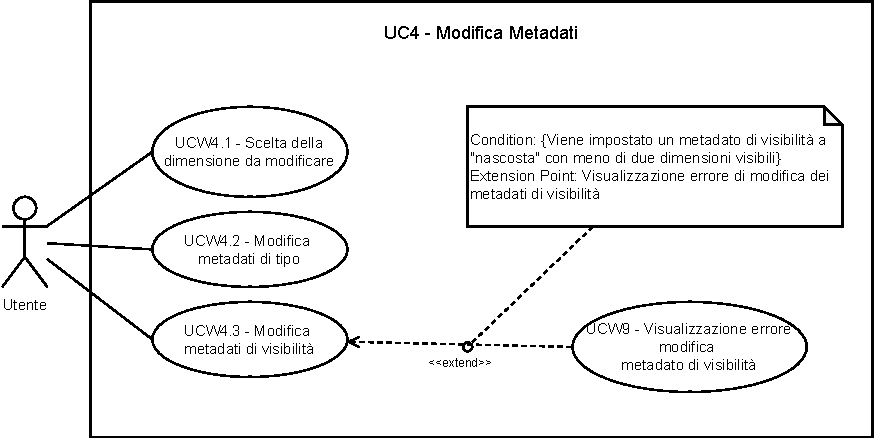
\includegraphics[width=0.8\textwidth]{diagrammi/UC4.pdf}
    \caption{Diagramma rappresentante UCW4}
    \label{fig:UCW4}
\end{figure}


\begin{itemize}
    \item \textbf{Descrizione}: L’utente modifica il grafico attuale del quale viene fornita la visualizzazione 
    aggiornata;

    \item \textbf{Attore primario}: Utente;

    \item \textbf{Precondizione}:   È stato costruito correttamente un grafico (\hyperref[sub:ucw2]{UCW2});

    \item \textbf{Postcondizione}:  Viene visualizzato il grafico modificato con i nuovi parametri;

	\item \textbf{Scenario principale}:
		\begin{enumerate}
            \item L'utente modifica i parametri di visualizzazione, interagendo con gli strumenti resi disponibili dal 
            grafico che sta visualizzando, dal menu di modifica;
            \item La visualizzazione del grafico viene aggiornata in accordo con i parametri modificati.
        \end{enumerate}

    \item \textbf{Scenari alternativi}:
    \begin{itemize}
        \item Annullamento delle modifiche:
        \begin{enumerate}
            \item L'utente seleziona la voce "Annulla" dal menù di modifica;
            \item Le modifiche vengono scartate e viene ripristinata la visualizzazione del grafico precedente 
            (\hyperref[ssub:ucw4.8]{UCW4.8}).
        \end{enumerate}
    \end{itemize}

\end{itemize}

\newpage
\subsubsection{UCW4.1 - Modifica grafico}
\label{ssub:ucw4.1}

\begin{itemize}
    \item \textbf{Descrizione}: L’utente effettua modifica specifiche al tipo di grafico precedentemente costruito e visualizzato,
                                su parametri quindi validi solo per tale visualizzazione, e ne vede le modifiche;

    \item \textbf{Attore primario}: Utente;

    \item \textbf{Precondizione}:   È stato costruito correttamente un grafico (\hyperref[sub:ucw2]{UCW2});

    \item \textbf{Postcondizione}:  Viene aggiornato il grafico costruito e visualizzato con i nuovi parametri;

    \item \textbf{Generalizzazioni}:
        \begin{itemize}
            \item Modifica Scatter Plot Matrix (\hyperref[ssub:ucw4.2]{UCW4.2});
            \item Modifica a grafico con Matrice delle Distanze (\hyperref[ssub:ucw4.3]{UCW4.3});
            \begin{itemize}
                \item Modifica Force Field (\hyperref[ssub:ucw4.4]{UCW4.4});
                \item Modifica Distance Map (\hyperref[ssub:ucw4.5]{UCW4.5});
             \end{itemize}
            \item Modifica Heat Map (\hyperref[ssub:ucw4.6]{UCW4.6});
            \item Modifica Proiezione Lineare Multi Asse (\hyperref[ssub:ucw4.7]{UCW4.7}).
        \end{itemize}
\end{itemize}

\subsubsection{UCW4.2 - Modifica Scatter Plot Matrix}
\label{ssub:ucw4.2}

\begin{figure}[h]
    \centering
    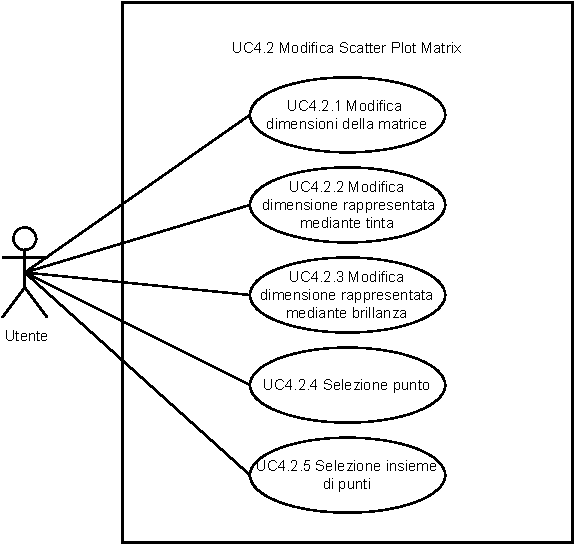
\includegraphics[width=0.6\textwidth]{diagrammi/UC4_2.pdf}
    \caption{Diagramma rappresentante UCW4.2}
    \label{fig:UCW4.2}
\end{figure}


\begin{itemize}
    \item \textbf{Descrizione}: L’utente modifica la visualizzazione dello Scatter Plot Matrix
                                costruito dal dataset corrente;

    \item \textbf{Attore primario}: Utente;

    \item \textbf{Precondizione}:   La visualizzazione costruita dal dataset corrente è uno Scatter Plot Matrix;

    \item \textbf{Postcondizione}:  Viene aggiornato il grafico costruito e visualizzato con i nuovi parametri;

	\item \textbf{Scenario principale}:
		\begin{enumerate}
            \item L'utente apporta le modifiche desiderate tra quelle offerte dallo Scatter Plot Matrix.
        \end{enumerate}
\end{itemize}


\paragraph{UCW4.2.1 - Modifica dimensioni della matrice}
\label{par:ucw4.2.1}
\begin{itemize}
    \item \textbf{Descrizione}:     L’utente dispone di dati con metadati assegnati e può
                                    scegliere fino a 5 dimensioni che possono essere visualizzate nello Scatter Plot
                                    Matrix;

    \item \textbf{Attore primario}: Utente;

    \item \textbf{Precondizione}:   La visualizzazione costruita dal dataset corrente è uno Scatter Plot Matrix;
    \item \textbf{Postcondizione}:  Vengono modificate le dimensioni visualizzate nei plot dello Scatter Plot Matrix;

	\item \textbf{Scenario principale}:
        \begin{enumerate}
            \item   L'utente seleziona l'opzione di selezione delle dimensioni;
            \item   L'utente seleziona fino a cinque dimensioni;

            \item   Ad ogni selezione l'utente
                    sceglie una delle dimensioni attuali del grafico e la scarta;

            \item   La visualizzazione sostituisce le dimensioni scartate con le nuove selezionate.
        \end{enumerate}
\end{itemize}

\paragraph{UCW4.2.2 - Modifica dimensione rappresentata mediante tinta}
\label{par:ucw4.2.2}
\begin{itemize}

    \item \textbf{Descrizione}:     L'utente assegna ad una dimensione un insieme di tinte per poterla rappresentare
                                    graficamente;

    \item \textbf{Attore primario}: Utente;
    \item \textbf{Precondizione}:   La visualizzazione correntemente costruita dal dataset è uno Scatter Plot Matrix;
    \item \textbf{Postcondizione}:  Viene aggiunta una dimensione rappresentata mediante tinta;
    \item \textbf{Scenario principale}:
    \begin{enumerate}

        \item   Interagendo con l'apposito pulsante, l'utente seleziona la dimensione che desidera rappresentare
                mediante tinta, sostituendo così quella precedente;

        \item   L'utente seleziona tra gli intervalli di tinte suggeriti quello con cui i diversi elementi della
                dimensione scelta saranno visualizzati;

        \item   La visualizzazione viene aggiornata in accordo con le modifiche effettuate.
    \end{enumerate}
\end{itemize}

\paragraph{UCW4.2.3 - Modifica dimensione rappresentata mediante brillanza}
\label{par:ucw4.2.3}
\begin{itemize}

    \item \textbf{Descrizione}:     L'utente assegna ad una dimensione la rappresentazione mediante brillanza;
    \item \textbf{Attore primario}: Utente;
    \item \textbf{Precondizione}:   La visualizzazione correntemente costruita dal dataset è uno Scatter Plot Matrix;
    \item \textbf{Postcondizione}:  Viene modificata la dimensione rappresentata mediante brillanza;
    \item \textbf{Scenario principale}:
    \begin{enumerate}
        \item   Interagendo con l'apposito pulsante, l'utente seleziona la dimensione che desidera rappresentare
                mediante brillanza, sostituendo così quella precedente;

        \item   La visualizzazione viene aggiornata in accordo con la modifica effettuata.
    \end{enumerate}
\end{itemize}

\paragraph{UCW4.2.4 - Selezione punto}
\label{par:ucw4.2.4}
\begin{itemize}
    \item \textbf{Descrizione}: L'utente seleziona un punto in uno Scatter Plot della matrice per vedere come
                                esso viene rappresentato negli altri grafici a dispersione della visualizzazione corrente;

    \item \textbf{Attore primario}: Utente;

    \item \textbf{Precondizione}:   La visualizzazione costruita dal dataset corrente è uno Scatter Plot Matrix;
    \item \textbf{Postcondizione}:  Le proiezioni del punto selezionato, se appartiene al dataset importato,
                                    vengono evidenziate in tutti i grafici della visualizzazione;

	\item \textbf{Scenario principale}:
        \begin{enumerate}
            \item L'utente seleziona un punto contente dati di uno Scatter Plot della matrice;
            \item La proiezione del punto viene evidenziata in tutti gli Scatter Plot della visualizzazione.
        \end{enumerate}

    \item \textbf{Scenari alternativi}:
    \begin{itemize}
        \item Selezione nulla:
        \begin{enumerate}
            \item L'utente seleziona un punto che non rappresenta nessun dato del dataset;
            \item Non viene evidenziato alcun punto della matrice.
        \end{enumerate}
    \end{itemize}

\end{itemize}


\paragraph{UCW4.2.5 - Selezione insieme di punti}
\label{par:ucw4.2.5}
\begin{itemize}
    \item \textbf{Descrizione}: L'utente seleziona un insieme di punti in uno Scatter Plot della matrice per vedere come
                                essi vengono rappresentati negli altri Scatterplot della matrice;

    \item \textbf{Attore primario}: Utente;

    \item \textbf{Precondizione}:   La visualizzazione costruita dal dataset corrente è uno Scatter Plot Matrix;
    \item \textbf{Postcondizione}:  Le proiezioni degli insiemi di punti selezionati, se appartenente al dataset importato,
                                    vengono evidenziate in tutti i grafici della visualizzazione;

	\item \textbf{Scenario principale}:
        \begin{enumerate}
            \item L'utente seleziona un insieme di punti di uno Scatter Plot della matrice;
            \item Le proiezioni dei punti contenenti dati vengono evidenziati in tutti gli Scatter Plot della visualizzazione.
        \end{enumerate}

    \item \textbf{Scenari alternativi}:
    \begin{itemize}
        \item Selezione nulla:
        \begin{enumerate}
            \item L'utente seleziona un insieme di punti vuoto;
            \item Non viene evidenziato alcun punto della matrice.
        \end{enumerate}
    \end{itemize}    

\end{itemize}

\newpage
\subsubsection{UCW4.3 - Modifica a grafico con matrice delle distanze}
\label{ssub:ucw4.3}

% TODO: Insert UC4.3 image
\begin{figure}[h]
    \centering
    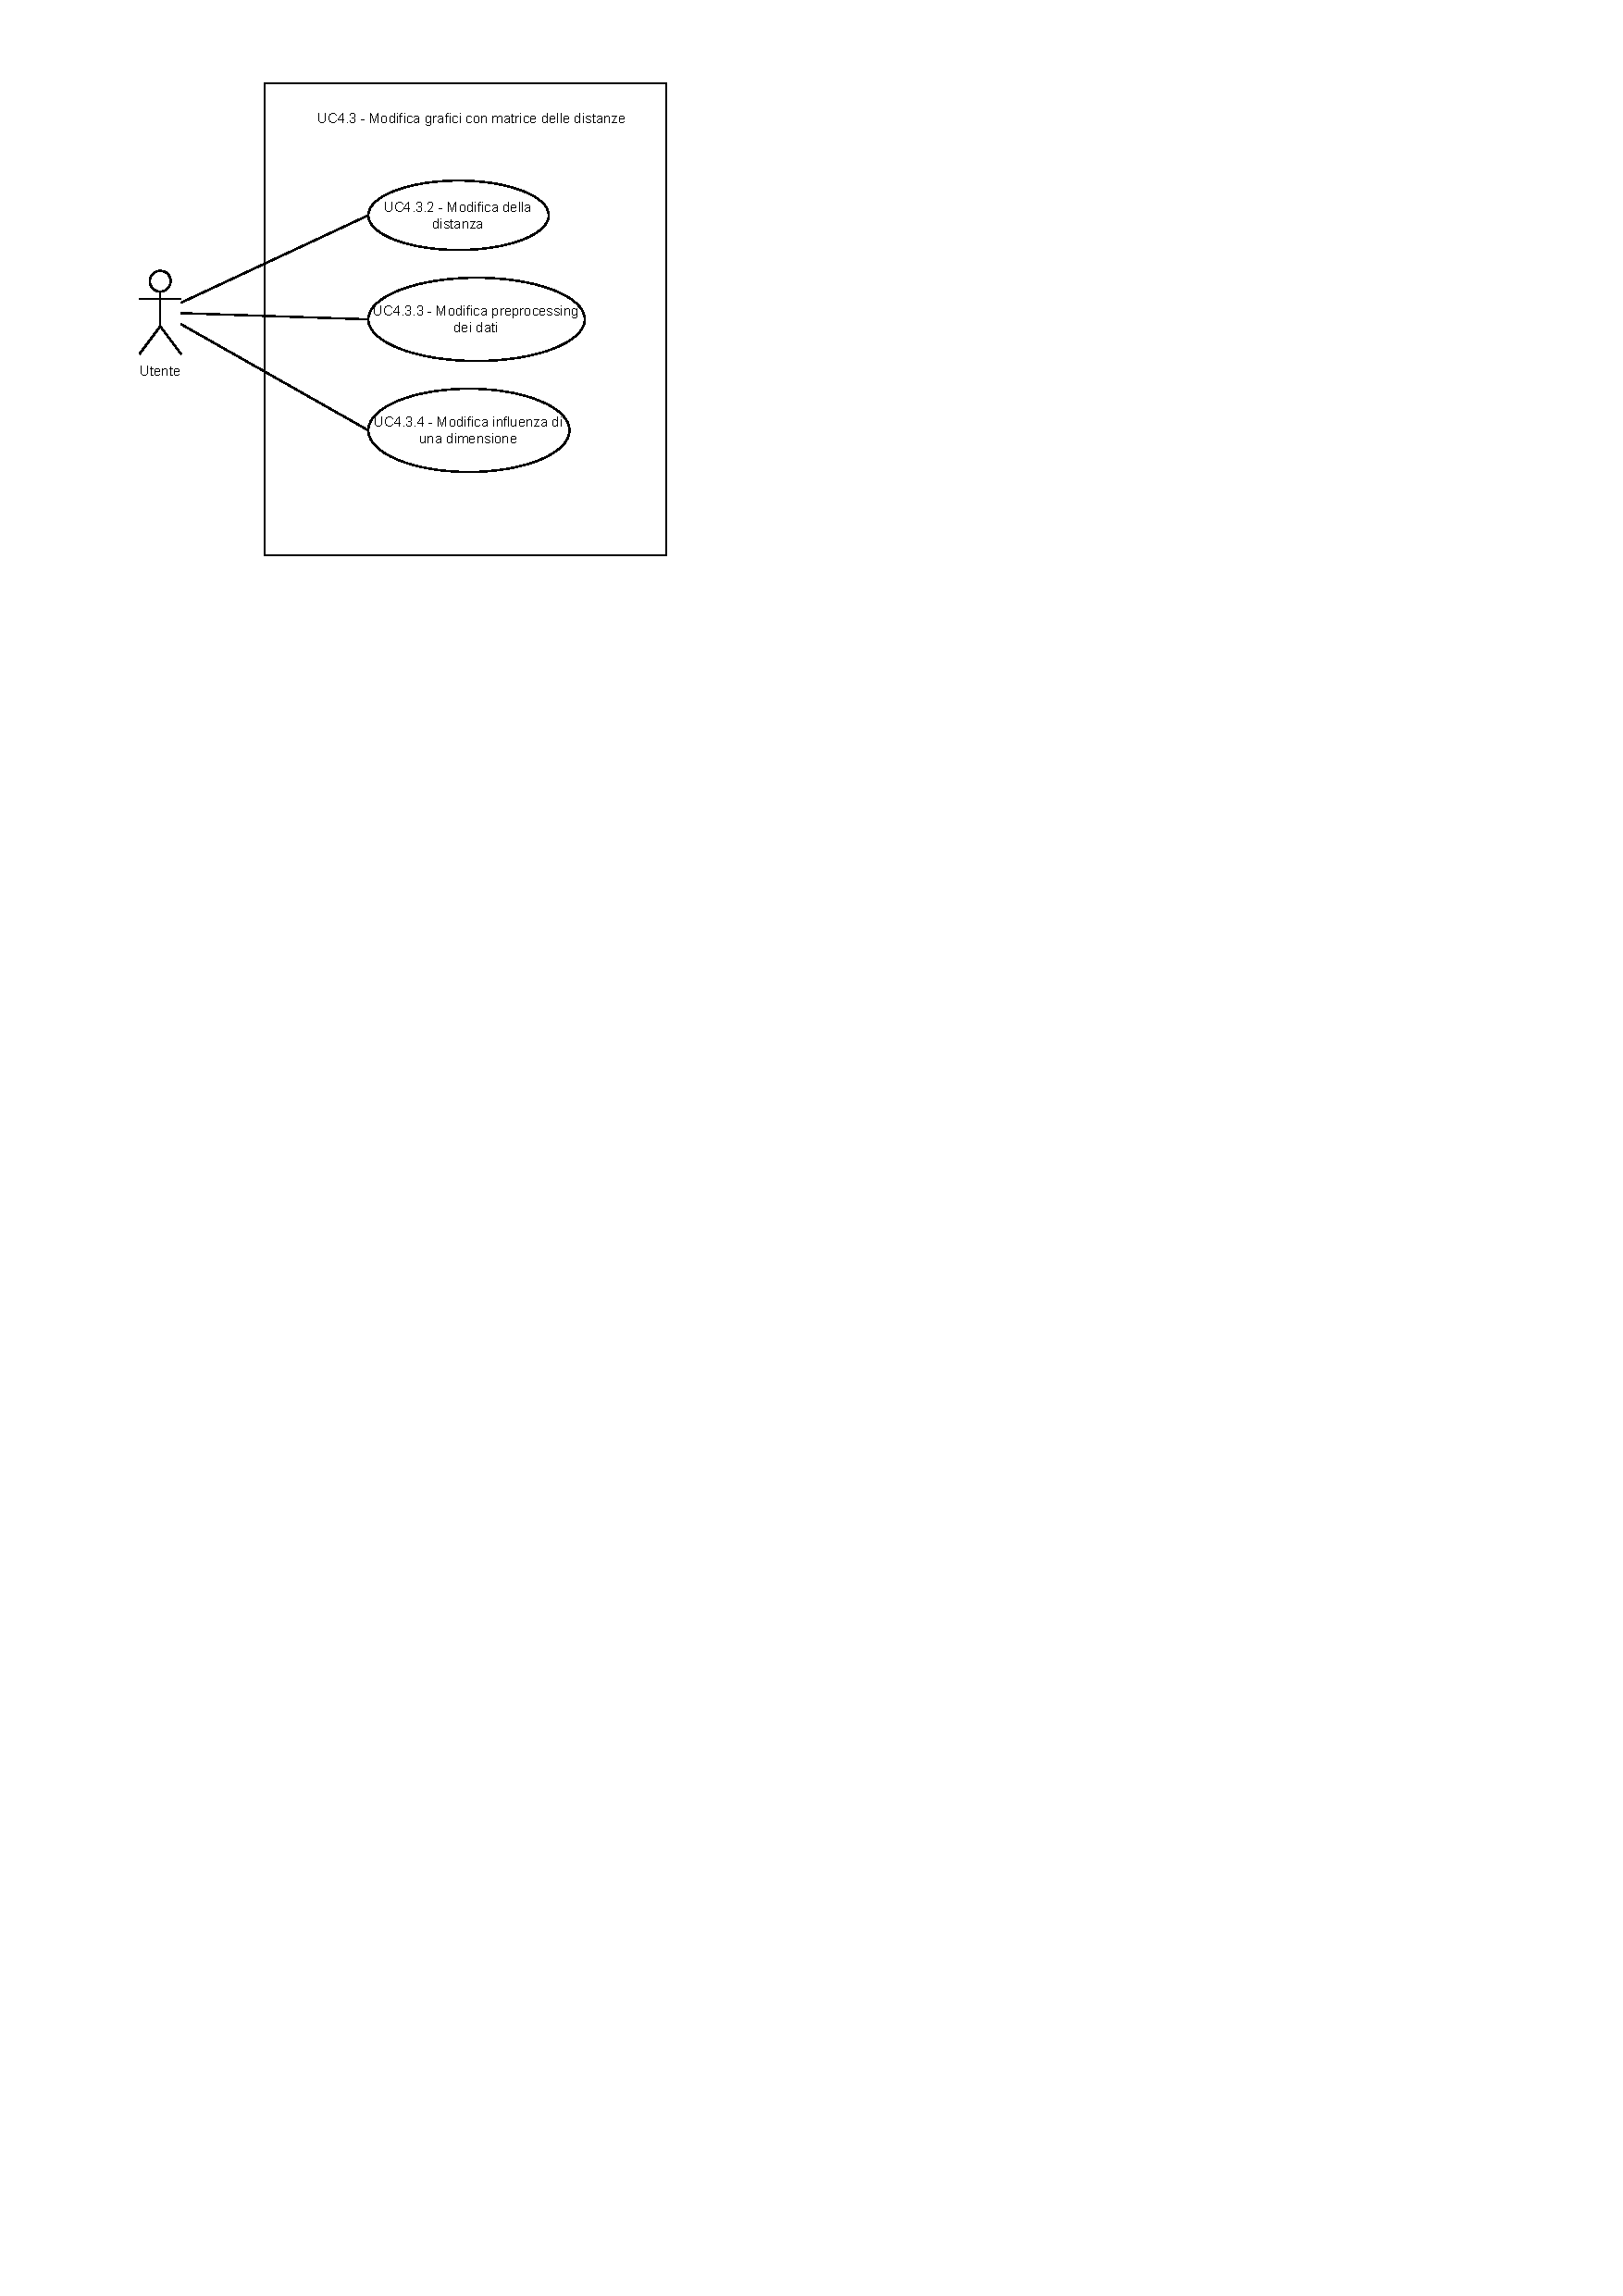
\includegraphics[width=0.8  \textwidth]{diagrammi/UC4_3.pdf}
    \caption{Diagramma rappresentante UCW4.3}
    \label{fig:UCW4.3}
\end{figure}

\begin{itemize}
    \item \textbf{Descrizione}: L’utente vuole modificare la visualizzazione di un grafico che sfrutta la matrice delle 
    distanze (Force Field e Distance Map) per la sua costruzione;
    \item \textbf{Attore primario}: Utente;
    \item \textbf{Precondizione}: La visualizzazione costruita dal dataset corrente è una Force Field o una Distance Map;
    \item \textbf{Postcondizione}: Viene aggiornato e visualizzato il grafico precedentemente costruito con i parametri opportunamente modificati;
    \item \textbf{Scenario principale}:
    \begin{enumerate}
        \item L’utente apporta le modifiche desiderate tra quelle offerte dai grafici costruiti tramite matrice delle 
        distanze e quelle specifiche al tipo di grafico attualmente costruito.
    \end{enumerate}
    \item \textbf{Generalizzazioni}:
    \begin{itemize}
        \item Modifica Force Field (\hyperref[ssub:ucw4.4]{UCW4.4});
        \item Modifica Distance Map (\hyperref[ssub:ucw4.5]{UCW4.5}).
    \end{itemize}
\end{itemize}

\paragraph{UCW4.3.1 - Modifica della distanza}
\label{par:ucw4.3.1}
\begin{itemize}
    \item \textbf{Descrizione}: L’utente decide di cambiare l’algoritmo usato per il calcolo delle distanze;

    \item \textbf{Attore primario}: Utente;

    \item \textbf{Precondizione}:   L'utente ha selezionato la voce \emph{"Modifica della distanza"} da (\hyperref[ssub:uc4.3]{UC4.3});
    \item \textbf{Postcondizione}:  La visualizzazione corrente viene aggiornata in funzione della matrice delle distanze ricalcolata;

	\item \textbf{Scenario principale}:
        \begin{enumerate}
            \item L'utente seleziona uno degli algoritmi di calcolo della distanza tra "\glossario{Euclidea}", 
            "\glossario{Manhattan}", "\glossario{Minkowski}", "\glossario{Canberra}";
            \item La distanza tra i punti viene ricalcolata secondo l'algoritmo scelto;
            \item La visualizzazione del grafico precedentemente costruito viene aggiornata.
        \end{enumerate}
\end{itemize}

\paragraph{UCW4.3.2 - Modifica preprocessing dei dati}
\label{par:ucw4.3.2}
\begin{itemize}
    \item \textbf{Descrizione}: L’utente sceglie se normalizzare, standardizzare o non effettuare alcuna operazione preliminare sui dati;

    \item \textbf{Attore primario}: Utente;
    \item \textbf{Precondizione}: L'utente ha selezionato la voce \emph{"Modifica preprocessing dei dati"} da (\hyperref[ssub:ucw4.3]{UCW4.3});
    \item \textbf{Postcondizione}: La visualizzazione corrente viene aggiornata in funzione della matrice delle distanze ricalcolata;
    \item \textbf{Scenario principale}:
    \begin{enumerate}
        \item L'utente seleziona la casella \emph{"Normalizza"} o \emph{"Standardizza"};
        \item HD Viz ricalcola la matrice delle distanze in base all'opzione scelta;
        \item La visualizzazione del grafico precedentemente costruito viene aggiornata.
    \end{enumerate}
\end{itemize}

\paragraph{UCW4.3.3 - Modifica influenza di una dimensione}
\label{par:ucw4.3.3}
\begin{itemize}
    \item \textbf{Descrizione}: Per visualizzare correttamente relazioni tra i dati,
                                l’utente decide di assegnare manualmente dei pesi alle dimensioni;

    \item \textbf{Attore primario}: Utente;
    \item \textbf{Precondizione}: L'utente ha selezionato la voce \emph{"Modifica influenza di una dimensione"} da (\hyperref[ssub:uc4.3]{UC4.3});

    \item \textbf{Postcondizione}: La visualizzazione corrente viene aggiornata in funzione della matrice delle distanze ricalcolata;
    \item \textbf{Scenario principale}:
    \begin{itemize}
        \item L’utente seleziona una dimensione del datset importato e le assegna manualmente un peso;
        \item HD Viz ricalcola la matrice delle distanze con i nuovi pesi;
        \item La visualizzazione del grafico precedentemente costruito viene aggiornata.
    \end{itemize}
\end{itemize}

\newpage
\subsubsection{UCW4.4 - Modifica Force Field}
\label{ssub:ucw4.4}
% TODO: Create image for force field graph.
\begin{figure}[h]
    \centering
    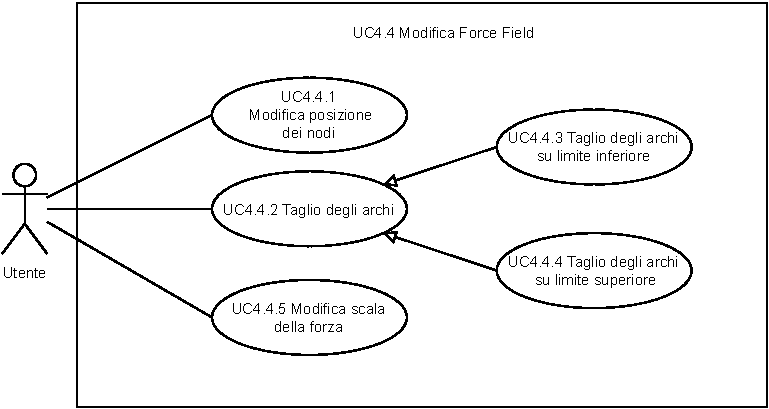
\includegraphics[width=0.6  \textwidth]{diagrammi/UC4_4.pdf}
    \caption{Diagramma rappresentante UCW4.4}
    \label{fig:UCW4.4}
\end{figure}


\begin{itemize}
    \item \textbf{Descrizione}: L’utente vuole modificare la visualizzazione del grafo Force Field
                                costruito dal dataset corrente;

    \item \textbf{Attore primario}: Utente;

    \item \textbf{Precondizione}:   La visualizzazione costruita dal dataset corrente è un Force Field;

    \item \textbf{Postcondizione}:  Viene aggiornato e visualizzato il grafico precedentemente costruito con i parametri opportunamente modificati;

    \item \textbf{Scenario principale}: 
    \begin{enumerate}
        \item L'utente apporta le modifiche desiderate tra quelle offerte dal Force Field.
    \end{enumerate}
\end{itemize}

\paragraph{UCW4.4.1 - Modifica posizione dei nodi}
\label{par:ucW4.4.1}
\begin{itemize}
    \item \textbf{Descrizione}: L’utente modifica la posizione dei nodi del grafo, trascinandoli nell'area definita dal grafico;

    \item \textbf{Attore primario}: Utente;

    \item \textbf{Precondizione}:   La visualizzazione costruita dal dataset corrente è un Force Field;
    \item \textbf{Postcondizione}:  Viene modificata la posizione dei nodi del grafo nella visualizzazione;

	\item \textbf{Scenario principale}:
        \begin{enumerate}
            \item L'utente clicca e trascina un nodo nello spazio della visualizzazione;
            \item La visualizzazione muove i punti del grafo mantenendo le connessioni tra i nodi.
        \end{enumerate}
\end{itemize}

\paragraph{UCW4.4.2 - Taglio degli archi}
\label{par:ucw4.4.2}
\begin{itemize}
    \item \textbf{Descrizione}:     L'utente imposta un valore di soglia sulla distanza e vengono eliminati gli archi che collegano nodi con distanza al di fuori della soglia impostata;
    \item \textbf{Attore primario}: Utente;
    \item \textbf{Precondizione}:   La visualizzazione correntemente costruita dal dataset è un Force Field;
    \item \textbf{Postcondizione}:  Viene aggiornata la visualizzazione, rimuovendo gli archi in base al valore di soglia impostato;
    \item \textbf{Scenario principale}:
    \begin{itemize}
        \item L'utente imposta una soglia;
        \item Vengono rimossi gli archi che collegano nodi che nella matrice delle distanze risultano avere una distanza che non rispetta la soglia impostata;
        \item La visualizzazione viene aggiornata con il grafo opportunamente aggiornato.
    \end{itemize}

    \item \textbf{Generalizzazioni}:
    \begin{itemize}
        \item Taglio degli archi su limite inferiore (\hyperref[par:ucw4.4.3]{UCW4.4.3});
        \item Taglio degli archi su limite superiore (\hyperref[par:ucw4.4.4]{UCW4.4.4}).
    \end{itemize}
\end{itemize}

\paragraph{UCW4.4.3 - Taglio degli archi su limite inferiore}
\label{par:ucw4.4.3}
\begin{itemize}
    \item \textbf{Descrizione}:     L'utente imposta il valore minimo della distanza e vengono eliminati gli archi che collegano nodi che nella matrice delle distanze hanno distanza minore al limite inferiore;
    \item \textbf{Attore primario}: Utente;
    \item \textbf{Precondizione}:   La visualizzazione correntemente costruita dal dataset è un Force Field;
    \item \textbf{Postcondizione}:  Viene aggiornata la visualizzazione rimuovendo gli archi  che collegano nodi tra loro distanti meno del valore di soglia minimo;
    \item \textbf{Scenario principale}:
    \begin{itemize}
        \item L'utente imposta il valore di soglia minimo;
        \item Vengono rimossi gli archi che collegano nodi che nella matrice delle distanze risultano avere una distanza inferiore alla soglia minima impostata;
        \item La visualizzazione viene aggiornata con il grafo opportunamente aggiornato.
    \end{itemize}
\end{itemize}

\paragraph{UCW4.4.4 - Taglio degli archi su limite superiore}
\label{par:ucw4.4.4}
\begin{itemize}
    \item \textbf{Descrizione}:     L'utente imposta il valore minimo della distanza e vengono eliminati gli archi che collegano nodi che nella matrice delle distanze hanno distanza maggiore al limite superiore;
    \item \textbf{Attore primario}: Utente;
    \item \textbf{Precondizione}:   La visualizzazione correntemente costruita dal dataset è un Force Field;
    \item \textbf{Postcondizione}:  Viene aggiornata la visualizzazione rimuovendo gli archi  che collegano nodi tra loro distanti più del valore di soglia massimo;
    \item \textbf{Scenario principale}:
    \begin{itemize}
        \item L'utente imposta il valore di soglia minimo;
        \item Vengono rimossi gli archi che collegano nodi che nella matrice delle distanze risultano avere una distanza superiore alla soglia massima impostata;
        \item La visualizzazione viene aggiornata con il grafo opportunamente aggiornato.
    \end{itemize}
\end{itemize}

\paragraph{UCW4.4.5 - Modifica scala della forza}
\label{par:ucw4.4.5}
\begin{itemize}
    \item \textbf{Descrizione}: L’utente decide di modificare la scala della forza di attrazione tra i nodi;


    \item \textbf{Attore primario}: Utente;

    \item \textbf{Precondizione}:   La visualizzazione correntemente costruita dal dataset è un Force Field;
    \item \textbf{Postcondizione}:  Viene modificata l'intensità della forza di attrazione tra i nodi del grafo nella visualizzazione.

	\item \textbf{Scenario principale}:
        \begin{enumerate}
            \item L'utente trascina il cursore sulla barra di intensità varia il valore dell’intensità;
            \item La visualizzazione modifica l'intensità della forza secondo il valore selezionato nel grafo;
            \item La visualizzazione viene aggiornata con il grafo opportunamente aggiornato.
        \end{enumerate}
\end{itemize}

\newpage
\subsubsection{UCW4.5 - Modifica Distance Map}
\label{ssub:ucw4.5}
% TODO: Insert image for Distance Map
\begin{figure}[h]
    \centering
    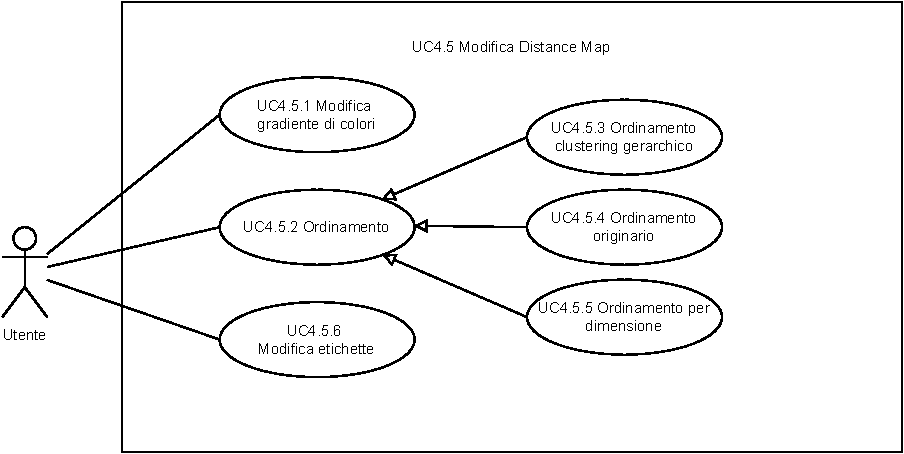
\includegraphics[width=0.8\textwidth]{diagrammi/UC4_5.pdf}
    \caption{Diagramma rappresentante UCW4.5}
    \label{fig:UCW4.5}
\end{figure}

\begin{itemize}
    \item \textbf{Descrizione}: L'utente vuole modificare la visualizzazione della Distance Map costruita dal dataset corrente;
    \item \textbf{Attore primario}: Utente;
    \item \textbf{Precondizione}: La visualizzazione costruita dal dataset corrente è un grafico di tipo Distance Map;
    \item \textbf{Postcondizione}: Viene aggiornato il grafico costruito con i nuovi parametri;
    \item \textbf{Scenario principale}:
    \begin{itemize}
        \item L'utente apporta le modifiche desiderate tra quelle offerte dalla Distance Map.
    \end{itemize}
\end{itemize}

\paragraph{UCW4.5.1 - Modifica gradiente di colori}
\label{par:ucw4.5.1}
\begin{itemize}
    \item \textbf{Descrizione}: L'utente decide di modificare la scala di colori applicata alla Distance Map scegliendo una tra le opzioni disponibili;
    \item \textbf{Attore primario}: Utente;
    \item \textbf{Precondizione}: La visualizzazione costruita dal dataset corrente è una Distance Map;
    \item \textbf{Postcondizione}: Viene modificata la scala dei colori del grafico nella visualizzazione;
    \item \textbf{Scenario principale}:
    \begin{itemize}
        \item L'utente seleziona la voce "Scala dei colori" e seleziona una tra le opzioni  "\glossario{Blue-Magenta-Yellow}", "\glossario{CoolWarm}", "\glossario{Dim Gray}";
        \item La visualizzazione cambia la scala dei colori adottata dalla Distance Map.
    \end{itemize}
\end{itemize}

\paragraph{UCW4.5.2 - Ordinamento}
\label{par:ucw4.5.2}
\begin{itemize}
    \item \textbf{Descrizione}: L'utente decide di ordinare le righe e le colonne del Distance Map al quale viene aggiunto un dendrogramma alla visualizzazione corrente;
    \item \textbf{Attore primario}: Utente;
    \item \textbf{Precondizione}: La visualizzazione costruita dal dataset corrente è una Distance Map;
    \item \textbf{Postcondizione}: Le righe e le colonne del Distance Map vengono visualizzate ordinate;
    \item \textbf{Scenario principale}:
    \begin{itemize}
        \item L'utente seleziona la casella di ordinamento;
        \item Le righe e le colonne della Distance Map vengono visualizzate secondo l'ordinamento selezionato;
    \end{itemize}
\end{itemize}

\paragraph{UCW4.5.3 - Ordinamento clustering gerarchico}
\label{par:ucw4.5.3}
\begin{itemize}
    \item \textbf{Descrizione}: L'utente decide di ordinare le righe e le colonne del Distance Map con l'algoritmo di clustering gerarchico il quale aggiunge un dendrogramma alla visualizzazione corrente;
    \item \textbf{Attore primario}: Utente;
    \item \textbf{Precondizione}: La visualizzazione costruita dal dataset corrente è una Distance Map;
    \item \textbf{Postcondizione}: Le righe e le colonne del Distance Map vengono visualizzate secondo l'ordine impostato dall'algoritmo di clustering gerarchico e con annesso il dendrogramma prodotto dall'ordinamento;
    \item \textbf{Scenario principale}:
    \begin{itemize}
        \item L'utente seleziona la casella di ordinamento delle colonne;
        \item Le righe e le colonne della Distance Map vengono visualizzate secondo l'ordinamento del clustering gerarchico e viene aggiunto il dendrogramma al grafico.
    \end{itemize}
\end{itemize}

\paragraph{UCW4.5.4 - Ordinamento originario}
\label{par:ucw4.5.4}
\begin{itemize}
    \item \textbf{Descrizione}: L'utente decide di ordinare le righe e le colonne del Distance Map seguendo l'ordine originario del dataset corrente;
    \item \textbf{Attore primario}: Utente;
    \item \textbf{Precondizione}: La visualizzazione costruita dal dataset corrente è una Distance Map;
    \item \textbf{Postcondizione}: Le righe e le colonne del Distance Map vengono visualizzate secondo l'ordine originario del dataset corrente;
    \item \textbf{Scenario principale}:
    \begin{itemize}
        \item L'utente seleziona la casella di ordinamento delle colonne;
        \item Le righe e le colonne della Distance Map vengono ordinate;
        \item Il grafico viene visualizzato aggiornato.
    \end{itemize}
\end{itemize}

\paragraph{UCW4.5.5 - Ordinamento per dimensione}
\label{par:ucw4.5.5}
\begin{itemize}
    \item \textbf{Descrizione}: L'utente decide di ordinare in maniera crescente le righe e le colonne del Distance Map secondo il valore delle dimensioni;
    \item \textbf{Attore primario}: Utente;
    \item \textbf{Precondizione}: La visualizzazione costruita dal dataset corrente è una Distance Map;
    \item \textbf{Postcondizione}: Le righe e le colonne del Distance Map vengono visualizzate ordinate secondo il valore delle dimensioni;
    \item \textbf{Scenario principale}:
    \begin{itemize}
        \item L'utente seleziona la casella di ordinamento delle colonne;
        \item Le righe e le colonne della Distance Map vengono ordinate;
        \item Il grafico viene visualizzato aggiornato.
    \end{itemize}
\end{itemize}


\paragraph{UCW4.5.6 - Modifica etichette}
\label{par:ucw4.5.6}
\begin{itemize}
    \item \textbf{Descrizione}: L'utente decide di modificare una etichetta associata alla Distance Map;
    \item \textbf{Attore primario}: Utente;
    \item \textbf{Precondizione}: La visualizzazione costruita dal dataset corrente è una Distance Map;
    \item \textbf{Postcondizione}: Le etichette della Distance Map vengono modificate secondo la scelta effettuata dall'utente;
    \item \textbf{Scenario principale}:
    \begin{itemize}
        \item L'utente sceglie una etichetta da modificare;
        \item L'utente sceglie una dimensione del dato da utilizzare come etichetta;
        \item Viene aggiornata l'etichetta nella Distance Map.
    \end{itemize}
\end{itemize}


\newpage
\subsubsection{UCW4.6 - Modifica Proiezione Lineare Multi Asse}
\label{ssub:ucw4.6}
% TODO: Create image for PLMA
\begin{figure}[h]
    \centering
    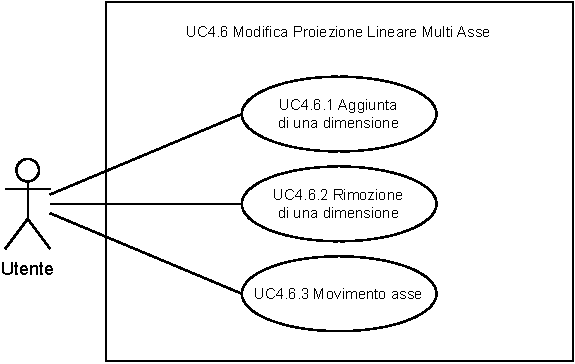
\includegraphics[width=0.8\textwidth]{diagrammi/UC4_6.pdf}
    \caption{Diagramma rappresentante UCW4.6}
    \label{fig:UCW4.6}
\end{figure}

\begin{itemize}
    \item \textbf{Descrizione}: L’utente vuole modificare la visualizzazione della Proiezione Lineare Multi Asse
                                costruita dal dataset corrente;

    \item \textbf{Attore primario}: Utente;

    \item \textbf{Precondizione}:   La visualizzazione costruita dal dataset corrente è un grafico di tipo Proiezione Lineare Multi Asse;
    \item \textbf{Postcondizione}:  Viene aggiornato il grafico costruito con i nuovi parametri;

	\item \textbf{Scenario principale}:
		\begin{enumerate}
            \item L'utente apporta le modifiche desiderate tra quelle offerte dalla Proiezione Lineare Multi Asse.
        \end{enumerate}
\end{itemize}

\paragraph{UCW4.6.1 - Aggiunta dimensione}
\label{par:ucw4.6.1}
\begin{itemize}
    \item \textbf{Descrizione}: L’utente aggiunge una dimensione del dataset importato al grafico;

    \item \textbf{Attore primario}: Utente;

    \item \textbf{Precondizione}:   La visualizzazione costruita dal dataset corrente è una Proiezione Lineare Multi Asse
                                    e rappresenta al più una dimensione in meno rispetto al numero di dimensioni del dataset;
    \item \textbf{Postcondizione}:  Alla visualizzazione della Proiezione Lineare Multi Asse viene aggiunta una dimensione;

	\item \textbf{Scenario principale}:
        \begin{enumerate}
            \item L'utente seleziona la voce "Dimensioni" e seleziona una dimensione da aggiungere alla proiezione;
            \item La visualizzazione aggiunge la dimensione selezionata e riposiziona i punti.
        \end{enumerate}
\end{itemize}

\paragraph{UCW4.6.2 - Rimozione dimensione}
\label{par:ucw4.6.2}
\begin{itemize}
    \item \textbf{Descrizione}: L’utente decide di rimuovere una dimensione dalla Proiezione Lineare Multi Asse
                                a patto che essa non sia monodimensionale;

    \item \textbf{Attore primario}: Utente;

    \item \textbf{Precondizione}:   La visualizzazione costruita dal dataset corrente è una Proiezione Lineare Multi Asse
                                    e rappresenta almeno due dimensioni;
    \item \textbf{Postcondizione}:  Alla visualizzazione della Proiezione Lineare Multi Asse viene rimossa una dimensione;

	\item \textbf{Scenario principale}:
        \begin{enumerate}
            \item L'utente seleziona la voce "Dimensioni" e seleziona una dimensione da rimuovere dalla proiezione;
            \item La visualizzazione rimuove la dimensione selezionata e riposiziona i punti.
        \end{enumerate}
\end{itemize}

\paragraph{UCW4.6.3 - Rotazione asse}
\label{par:ucw4.6.3}
\begin{itemize}
    \item \textbf{Descrizione}: L'utente ruota gli assi nella visualizzazione per visualizzare diverse proiezioni dello stesso dataset;
    \item \textbf{Attore primario}: Utente;
    \item \textbf{Precondizione}: La visualizzazione costruita dal dataset corrente è una Proiezione Lineare Multi Asse;
    \item \textbf{Postcondizione}: Il grafico viene ridisegnato con gli assi opportunamente ruotati;
    \item \textbf{Scenario principale}:
    \begin{enumerate}
        \item L'utente trascina un asse del grafico ruotandolo;
	    \item La visualizzazione viene aggiornata con l'asse ruotandolo.
    \end{enumerate}
\end{itemize}

\newpage

\subsubsection{UCW4.7 - Modifica Heat Map}
\label{ssub:ucw4.7}
% TODO: Create image for force field graph.
\begin{figure}[h]
    \centering
    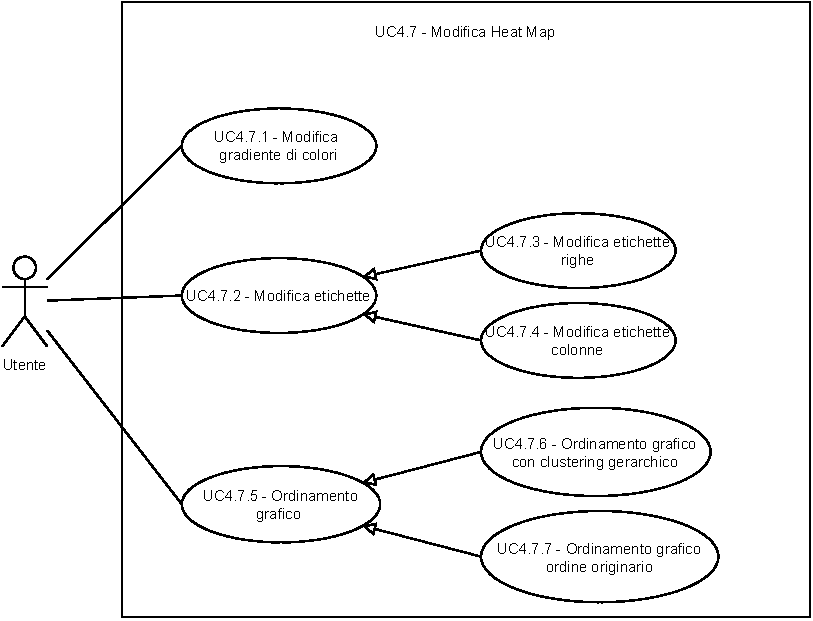
\includegraphics[width=0.6\textwidth]{diagrammi/UC4_7.pdf}
    \caption{Diagramma rappresentante UCW4.7}
    \label{fig:UCW4.7}
\end{figure}


\begin{itemize}
    \item \textbf{Descrizione}: L’utente modifica la visualizzazione della Heat Map correntemente visualizzata;

    \item \textbf{Attore primario}: Utente;

    \item \textbf{Precondizione}:   La visualizzazione correntemente costruita dal dataset è una Heat Map;

    \item \textbf{Postcondizione}:  Viene aggiornata la visualizzazione secondo i nuovi parametri impostati;

	\item \textbf{Scenario principale}:
		\begin{enumerate}
            \item L'utente apporta le modifiche desiderate tra quelle offerte dalla Heat Map.
        \end{enumerate}
\end{itemize}

\paragraph{UCW4.7.1 - Modifica gradiente di colori}
\label{par:ucw4.7.1}
\begin{itemize}
    \item \textbf{Descrizione}: L'utente decide di modificare la scala di colori applicata alla Heat Map scegliendo una tra le opzioni disponibili;

    \item \textbf{Attore primario}: Utente;

    \item \textbf{Precondizione}:   La visualizzazione costruita dal dataset corrente è una Heat Map;
    \item \textbf{Postcondizione}:  Viene modificata la scala dei colori del grafico nella visualizzazione;

	\item \textbf{Scenario principale}:
        \begin{enumerate}
            \item L'utente seleziona la voce "Scala dei colori" e seleziona una tra le opzioni  "\glossario{Blue-Magenta-Yellow}", "\glossario{CoolWarm}", "\glossario{Dim Gray}";
            \item La visualizzazione cambia la scala dei colori adottata dalla Heat Map.
        \end{enumerate}
\end{itemize}

\paragraph{UCW4.7.2 - Modifica etichette delle righe}
\label{par:ucw4.7.3}
\begin{itemize}
    \item \textbf{Descrizione}:     L'utente modifica l'etichetta associata alle righe della Heat Map;
    \item \textbf{Attore primario}: Utente;
    \item \textbf{Precondizione}:   La visualizzazione correntemente costruita dal dataset è una Heat Map;
    \item \textbf{Postcondizione}:  Le etichette delle righe dell'Heat Map vengono modificate secondo la scelta effettuata dall'utente;
    \item \textbf{Scenario principale}:
    \begin{enumerate}
        \item L'utente sceglie una etichetta da modificare;
        \item L'utente sceglie una dimensione del dato da utilizzare come etichetta;
        \item Viene aggiornata l'etichetta nella Distance Map.
    \end{enumerate}
\end{itemize}

\paragraph{UCW4.7.3 - Modifica etichette delle colonne}
\label{par:ucw4.7.4}
\begin{itemize}
    \item \textbf{Descrizione}:     L'utente modifica l'etichetta associata alla colonna della Heat Map;
    \item \textbf{Attore primario}: Utente;
    \item \textbf{Precondizione}:   La visualizzazione correntemente costruita dal dataset è una Heat Map;
    \item \textbf{Postcondizione}:  Le etichette delle colonne dell'Heat Map vengono modificate secondo la scelta effettuata dall'utente;
    \item \textbf{Scenario principale}:
    \begin{enumerate}
        \item L'utente sceglie una etichetta da modificare;
        \item L'utente sceglie una dimensione del dato da utilizzare come etichetta;
        \item Viene aggiornata l'etichetta nella Distance Map.
    \end{enumerate}
\end{itemize}

\paragraph{UCW4.7.4 - Ordinamento grafico}
\label{par:ucw4.7.5}
\begin{itemize}
    \item \textbf{Descrizione}:     L'utente modifica l'ordinamento delle colonne della visualizzazione;
    \item \textbf{Attore primario}: Utente;
    \item \textbf{Precondizione}:   La visualizzazione correntemente costruita dal dataset è una Heat Map;
    \item \textbf{Postcondizione}:  L'ordine delle colonne viene modificato;
    \item \textbf{Scenario principale}:
    \begin{enumerate}
        \item L'utente seleziona uno tra i possibili ordinamenti delle colonne;
        \item L'ordinamento del grafico viene modificato in base a quanto precedentemente selezionato.
    \end{enumerate}
    \item \textbf{Generalizzazioni}:
    \begin{itemize}
        \item Ordinamento clustering gerarchico (\hyperref[spar:ucw4.7.5]{UCW4.7.5});
        \item Ordinamento secondo ordine originario (\hyperref[spar:ucw4.7.6]{UCW4.7.6}).
    \end{itemize}
\end{itemize}

\subparagraph{UCW4.7.5 - Ordinamento grafico mediante clustering gerarchico}
\label{spar:ucw4.7.5}
\begin{itemize}
    \item \textbf{Descrizione}:     L'utente modifica l'ordinamento del grafico  della visualizzazione secondo l'algoritmo di clustering gerarchico;
    \item \textbf{Attore primario}: Utente;
    \item \textbf{Precondizione}:   La visualizzazione correntemente costruita dal dataset è una Heat Map;
    \item \textbf{Postcondizione}:  L'ordine delle colonne viene modificato in accordo con il risultato dell'applicazione dell'algoritmo di clustering gerarchico;
    \item \textbf{Scenario principale}:
    \begin{enumerate}
        \item L'utente seleziona l'ordinamento delle colonne con clustering gerarchico;
        \item L'ordinamento delle colonne della visualizzazione viene modificato in base al risultato dell'algoritmo di clustering gerarchico;
        \item Viene aggiunto sull'asse orizzontale il dendrogramma associato alla clusterizzazione.
    \end{enumerate}
\end{itemize}

\subparagraph{UCW4.7.6 - Ordinamento grafico secondo ordine originario }
\label{spar:ucw4.7.6}
\begin{itemize}
    \item \textbf{Descrizione}:     L'utente modifica l'ordinamento del grafico secondo l'ordine in cui i dati sono disposti nel dataset;
    \item \textbf{Attore primario}: Utente;
    \item \textbf{Precondizione}:   La visualizzazione correntemente costruita dal dataset è una Heat Map ed è stato selezionato il bottone "Ordina" all'interno del campo "Colonne";
    \item \textbf{Postcondizione}:  L'ordine delle colonne viene modificato in accordo con il risultato dell'applicazione dell'algoritmo di clustering gerarchico;
    \item \textbf{Scenario principale}:
    \begin{enumerate}
        \item L'utente seleziona l'ordinamento delle colonne con clustering gerarchico;
        \item L'ordinamento delle colonne della visualizzazione viene modificato in base al risultato dell'algoritmo di clustering gerarchico;
        \item Viene aggiunto sull'asse orizzontale il dendrogramma associato alla clusterizzazione.
    \end{enumerate}
\end{itemize}



\subsubsection{UCW4.8 - Annullamento delle modifiche}
\label{ssub:ucw4.8}
\begin{itemize}
    \item \textbf{Descrizione}: L'utente decide di scartare le modifiche fatte nella corrente selezione di modifica;

    \item \textbf{Attore primario}: Utente;

    \item \textbf{Precondizione}:   L'utente ha selezionato la voce di Modifica Grafico dal menù;
    \item \textbf{Postcondizione}:  Viene ripristinato il grafo ai parametri precedenti della selezione e visualizzato;

	\item \textbf{Scenario principale}:
        \begin{enumerate}
            \item L'utente seleziona il pulsante "Annulla modifiche";
            \item HD Viz ripristina i parametri del grafo ai valori precedenti alla selezione del menu di modifica.
        \end{enumerate}
\end{itemize}
